\documentclass[letterpaper]{article}

\usepackage{natbib,alifeconf}  %% The order is important
\usepackage{url,hyperref,cleveref}
\usepackage{booktabs}

% *****************
%  Requirements:
% *****************
%
% - All pages sized consistently at 8.5 x 11 inches (US letter size).
% - PDF length <= 8 pages for full papers, <=2 pages for extended
%    abstracts (not including citations).
% - Abstract length <= 250 words.
% - No visible crop marks.
% - Images at no greater than 300 dpi, scaled at 100%.
% - Embedded open type fonts only.
% - All layers flattened.
% - No attachments.
% - All desired links active in the files.

% Note that the PDF file must not exceed 5 MB if it is to be indexed
% by Google Scholar. Additional information about Google Scholar
% can be found here:
% http://www.google.com/intl/en/scholar/inclusion.html.


% If your system does not generate letter format documents by default,
% you can use the following workflow:
% latex example
% bibtex example
% latex example ; latex example
% dvips -o example.ps -t letterSize example.dvi
% ps2pdf example.ps example.pdf


% For pdflatex users:
% The alifeconf style file loads the "graphicx" package, and
% this may lead some users of pdflatex to experience problems.
% These can be fixed by editing the alifeconf.sty file to specify:
% \usepackage[pdftex]{graphicx}
%   instead of
% \usepackage{graphicx}.
% The PDF output generated by pdflatex should match the required
% specifications and obviously the dvips and ps2pdf steps become
% unnecessary.


% Note:  Some laser printers have a serious problem printing TeX
% output. The use of ps type I fonts should avoid this problem.


% \title{ALIFE2024 template}



\title{SSIE 583 Project: \\Generating Look-up tables from Partial Input Data in CANA\\}
% Each submission will undergo a double-blind review process. To this end, submissions should NOT contain any element that could reveal the identity of the authors (author names, affiliations, funding details and acknowledgments), and should use the third person to refer to previous work by the authors.
\author{
    Srikanth Iyer%$^{1}$,
    % Second Author$^{1,2}$, \and
    % Third Author$^2$ \\
    % \mbox{}
    \\
    % $^1$
    Thomas J. Watson College of Engineering and Applied Science, Binghamton University, SUNY, USA \\
    siyer5@binghamton.edu\\\\
    \today
    % $^2$Second Institution Name, Second Institution Country
    % correspondin-author@email.com
} % email of corresponding author


% For several authors from the same institution use the same number to
% refer to one address.
%
% If the names do not fit well on one line use
%         Author 1, Author 2 ... \\ {\Large\bf Author n} ...\\ ...
%
% If the title and author information do not fit in the area
% allocated, place \setlength\titlebox{<new height>} after the
% \documentclass line where <new height> is 2.25in



\begin{document}

\maketitle

\begin{abstract}
    This paper discusses the addition of a new feature to the CANA package, which allows the generation of lookup tables from incomplete data. The current implementation of CANA assumes complete input data, but in real-world scenarios, it is often not possible to provide all the necessary inputs. The goal of this project is to extend the capabilities of CANA to handle partial, or incomplete data to facilitate the identification of gaps and contradictions, and evaluation of the statespace of the boolean network from existing knowledge status. The paper also discusses some issues encountered during the implementation and suggests future work, including incorporating bias into the lookup table generation function. Overall, the addition of the ability to generate lookup tables from incomplete data enhances the usability and robustness of the CANA package, making it a valuable tool for studying and analyzing complex systems in computational biology and systems biology.
\end{abstract}




\section{Introduction}

CANA: A Python Package for Quantifying Control and Canalization in Boolean Networks \citep{CANA} is a powerful tool designed to extract, measure, and visualize canalizing redundancy and effective pathways in controlling dynamics present in Boolean network models.
It does so with tools such as the 'effective graph' and 'dynamics canalizing map' as well as others to 'uncover minimum sets of control variables', which are important for controlling and manipulating biological systems. 
This makes CANA a valuable tool for studying and analyzing complex systems in the field of computational biology and systems biology. 

While effective graphs and two-symbol schemata allow us to boil down the output rules to its bare essentials and capture relationships hidden in redundancies, this paper will focus on an addition made to the toolkit of CANA- the ability to generate look-up tables from partially described boolean networks. 
This feature allows users to efficiently interpolate and extrapolate data points, identifying gaps in input data, and potential contradictions in the lookup table. 


\section{Background}
Currently, CANA has two types of inputs that instantiate a Boolean Node in a Boolean Network.

The \textbf{lookup table input}- a list of 2-tuples, where the first element is a binary string of length $k$ and the second element is a binary string of length $1$. 
For example, the lookup table input for a node with $k=2$ would look like this: Table(\ref{table:boolean-input})

    \begin{table}
        \centering
        \begin{tabular}{|c|c|}
            \hline
            Input & Output \\
            \hline
            000 & 0 \\
            001 & 1 \\
            010 & 0 \\
            011 & 1 \\
            100 & 0 \\
            101 & 1 \\
            110 & 0 \\
            111 & 1 \\
            \hline
        \end{tabular}
        \caption{Example Boolean Input for Three Inputs}
        \label{table:boolean-input}
    \end{table}
\textbf{Prime Implicants (PI)}: The CANA package also accepts a partial input, where the user can generate a complete lookup table by specifying just the Prime Implicants (PI). See: Table (\ref{table:boolean-input-PI}). 
Currently, when instantiating a boolean node in the boolean network, the package will assume an output value of '0' for all unspecified inputs. 
This is a reasonable assumption, as the lookup table is a complete representation of the node's behavior. 
Assuming the completeness of the input data allows the package to find Prime Implicants sufficient to generate the entire lookup table.
    \begin{table}
        \centering
        \begin{tabular}{|c|c|}
            \hline
            Input & Output \\
            \hline
            \#\#1 & 1 \\
            \hline
        \end{tabular}
        \caption{Alternative view of table: (\ref{table:boolean-input}) inputs with only Prime Implicants. The '\#' symbol is a 'don't care' symbol.}
        \label{table:boolean-input-PI}
    \end{table}
Similarly, \Cref{fig:thaliana-LFY-input-PI} is an example of the Prime Implicant inputs for the LFY node in Arabidopsis Thaliana.
This generates the lookup-table in \Cref{fig:thaliana-LFY-lookuptable}. 
\begin{figure}[h]
    \centering
    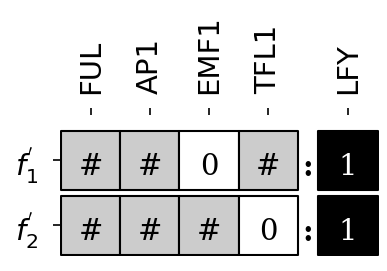
\includegraphics[width=0.3\textwidth]{thalianaLFY.png}
    \caption{Prime Implicants input \citep{CANA} for the LFY gene in Arabidopsis Thaliana \citep{thaliana}. The '\#' symbol is a 'don't care' symbol.}
    \label{fig:thaliana-LFY-input-PI}
\end{figure}

\begin{figure}[ht]
    \centering
    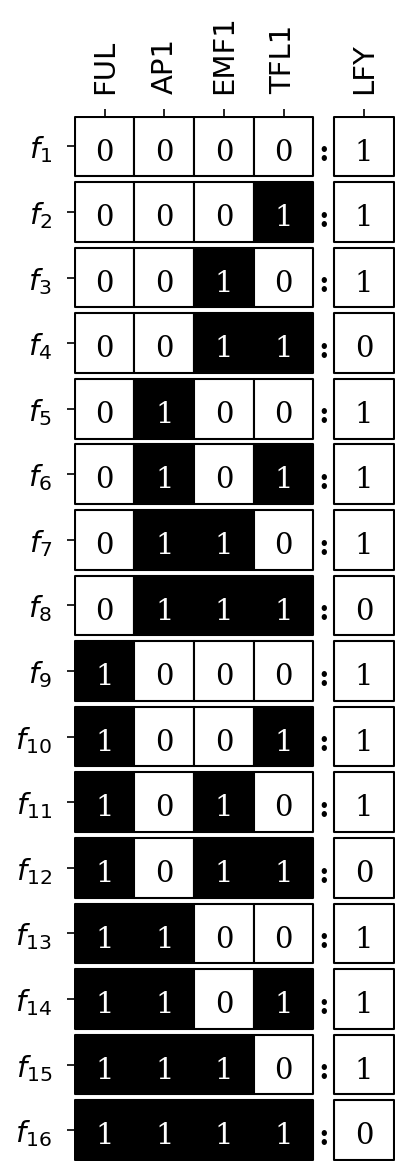
\includegraphics[width=0.25\textwidth]{thalianaLFYlookuptable.png}
    \caption{The complete lookup table for the LFY gene in Arabidopsis Thaliana.}
    \label{fig:thaliana-LFY-lookuptable}
\end{figure}

\section{Problem Statement}
The current implementation of CANA assumes that the lookup table is complete, and the user has provided all the necessary inputs. 
However, in real-world scenarios, it is not always possible to provide all the inputs.
The scientific process is one that is full of uncomfortable interactions with reality- where models and abstractions have to perform in the arena of truth. 
The truth is not only stern, but also oft elusive.
Our understanding of interactions between nodes within bio-regulatory networks relies heavily on rigorous scientific experimentation. 
These hard-won insights provide the foundation for Boolean Networks, which can then be used to process information and advance our knowledge of these complex systems.
It also means that the data we have is often incomplete, noisy, or uncertain.
Generating lookup tables from partial data will give us a better understanding of the data we have, what it tells us, and what it doesn't. 
It will also help us identify gaps in our data, and potentially identify contradictions in the data we have.

\section{Generating Tables from Incomplete Data}
The goal of this project is to extend the capabilities of CANA to generate lookup tables from the partial data available to the user. 
To do this, we will need to:
\begin{itemize}
    \item Make no assumptions about the completeness of the data. This is done by assigning a value of '?' instead of '0' to all unspecified inputs.
    \item Parsing input for 'don't care' symbols ('\#','--', etc). Iterating all combinations of the boolean values for each symbol and assigning the provided output value to them.
    \item Identify gaps in the data provided by the user. 
    \item Generating missing input values, assigning the '?' output to them. This will communicate the information-completeness of the boolean network to the user.
    \item Identify contradictions in the data provided by the user. The current implementation of CANA assumes that there are no contradiction in the data- due to the completeness assumption of the inputs. Contradictory outputs are flagged with a '!' symbol.
    \item Generate the lookup table from the data provided by the user.    
\end{itemize}
With incomplete inputs, including 'don't care' symbols such as the example in \Cref{table:tempynode5-input}, the lookup table generated by CANA will look like the one in \Cref{fig:tempynode5-lookuptable}.



\begin{table}
    \centering
    \begin{tabular}{|c|c|}
        \hline
         Input  & Output \\
        \hline
        00\#\# & 0 \\
        1\#\#1 & 1 \\
        11\#\# & 0 \\
        \hline
    \end{tabular}
    \caption{Incomplete and contradictory input example. The '\#' symbol represents 'don't care' inputs.}
    \label{table:tempynode5-input}
\end{table}


\begin{figure}
    \centering
    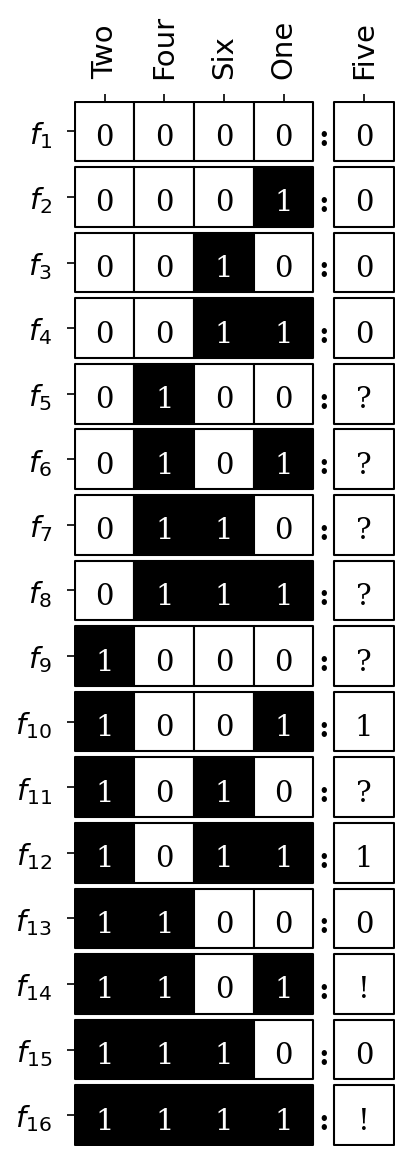
\includegraphics[width=0.25\textwidth]{tempynode5lookuptable.png}
    \caption{The complete lookup table for Example input from \Cref{table:tempynode5-input}. The '?' indicates missing input data. The '!' indicates contradictory output values for the given (or permuted) input.}
    \label{fig:tempynode5-lookuptable}
\end{figure}

\section{Issues Encountered and Future Work}
While this addition to the CANA package is a step in the right direction, there are still some issues that need to be addressed. 
With every addition to the package, the probability of unexpected breakages increases. 

\begin{itemize}
    \item The current implementation doesn't account for Prime Implicants as inputs. 
    This is a significant oversight on my part, as the package already has the capability to generate lookup tables from Prime Implicants and the new addition depreciates this feature.
    I will need to address this issue in the next iteration of the package.
    \item The styles of input in the datasets in the package vary, which makes discerning the intentions behind the data styles a challenge for me. 
    Evaluating the input txt files to make it more parsable: either in json or csv format can be a potential solution to this issue.
    \item To distinguish between inputs that are complete and in the form of Prime Implicants and inputs that are incomplete will require further clarification either from the user or in the dataset documentation itself. 
    As of now, deducing this purely from the input values given is proving a challenge. 
    This could be either due to the lack of understanding, or coding inexperience, or it could be an issue that needs to be addressed in future implementations of CANA for the sake of internal consistency of the package and intuitive usability. Ideally, there should be a way to deduce and distinguish both types of data without requiring the user to specify it. This will be my immediate focus on the project. 
    \item Investigating all other potential breakages in the package will be the next step. This includes looking and for more edge cases and testing the package with more datasets .
    \item Applying Bias to the lookup table generation function will enable the user to generate lookup tables that are more in line with their expectations.
\end{itemize}

\section{Conclusion}
The addition of the ability to generate lookup tables from incomplete data is a useful addition to the CANA package.
It allows users to better understand the data they have, identify gaps in their data, and potentially identify contradictions in the data they have.
It will also allow the ability to evaluate the statespace of the boolean network, and identify the states that are unreachable, or likely from the given partial data.
Incorporating more features such as biasing the generated table, and automatically distinguishing between Prime Implicants and incomplete data will enable the package to be more user-friendly, intuitive, and robust.
This will be the focus of the next iteration of the package.

\section{Acknowledgements}
I would like to thank Dr. Rocha for the project idea. 
Learning CANA facilitates learning more about boolean networks and graphs, which is a good foundation for understanding complex systems.
I would also like to thank Dr Rozum for handholding me through the CANA package, and his suggestions for future implementation.
Thank you for your time and consideration. This work is nowhere near completion and I'm looking forward to finishing it in the near future. 

\footnotesize



\bibliographystyle{apalike}
\bibliography{example} % replace by the name of your .bib file
\end{document}